\chapter{Further Material}

\section{Interpolation}
\begin{my_figure}[!h]{width=1\textwidth}{interpol/2x3_loess_robust}
	\caption{The LOESS smoother \RobItPlot}
	\label{fig:interpol/2x3_loess_robust}
\end{my_figure}

\begin{my_figure}[!h]{width=1\textwidth}{interpol/2x3_B-Splines_robust}
	\caption{B-Splines \RobItPlot}
	\label{fig:interpol/2x3_B-Splines_robust}
\end{my_figure}

\begin{my_figure}[!h]{width=1\textwidth}{interpol/2x3_DL_robust}
	\caption{A Double Logistic curve \RobItPlot}
	\label{fig:interpol/2x3_DL_robust}
\end{my_figure}




\section{NDVI correction}
\todo[inline]{page breaks}

% step_plot/2017-201_ndvi.pdf 
% step_plot/2017-202_itpl.pdf 
% step_plot/2017-203_itpl_rew.pdf 
% step_plot/2017-204_ndvi_scl.pdf 
% step_plot/2017-205_show_res.pdf 
% step_plot/2017-206_corr.pdf 
% step_plot/2017-207_uncert.pdf 
% step_plot/2017-208_corr_itpl_rew.pdf

\begin{figure}[H]
	% \vspace{-15pt}
	% \centering
	% \begin{subfigure}[b]{0.42\textwidth}
	% 	\centering
	% 	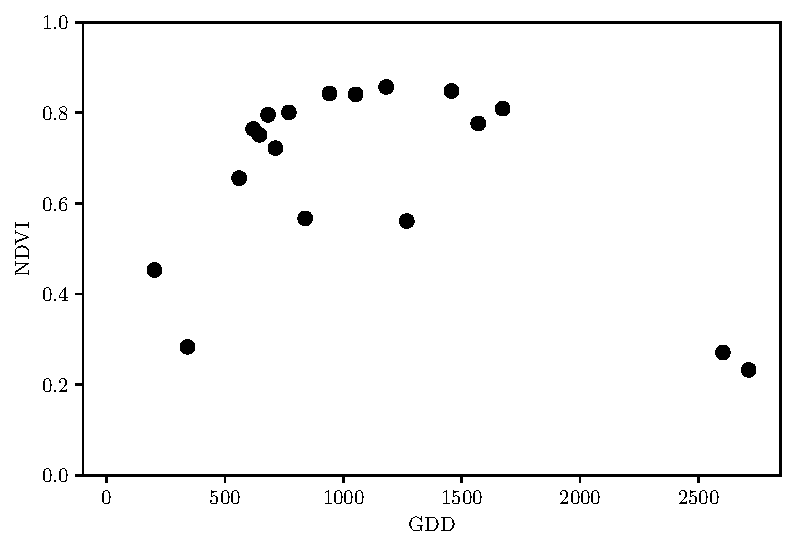
\includegraphics[width=\textwidth]{step_plot/2017-201_ndvi.pdf}
	% 	\vspace{-20pt}
	% 	\caption[NDVI {TS} with SCL45]%
	% 	{{\footnotesize NDVI {TS} with SCL45}}    
	% 	\label{fig:step_plot/2017-201_ndvi.pdf}
	% \end{subfigure}
	% \hfill
	
	\vskip\baselineskip
	\begin{subfigure}[b]{0.42\textwidth}  
		\centering 
		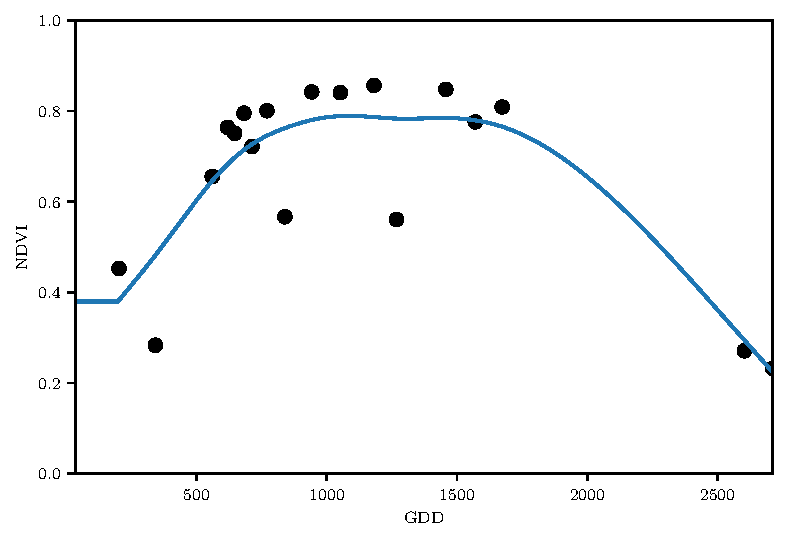
\includegraphics[width=\textwidth]{step_plot/2017-202_itpl.pdf}
		\vspace{-20pt}
		\caption[Interpolation via SS (only SCL45)]%
		{{\footnotesize Interpolation via SS (only SCL45)}}    
		\label{fig:step_plot/2017-202_itpl.pdf}
	\end{subfigure}
	% \begin{subfigure}[b]{0.42\textwidth}   
	% 	\centering 
	% 	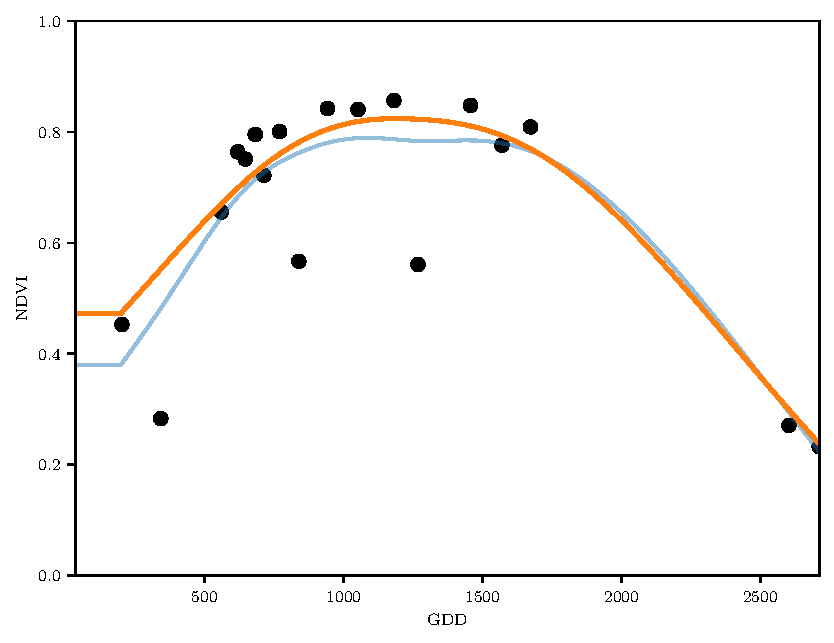
\includegraphics[width=\textwidth]{step_plot/2017-203_itpl_rew.pdf}
	% 	\vspace{-20pt}
	% 	\caption[Robustly reweighted fit]%
	% 	{{\footnotesize Robustly reweighted fit}}    
	% 	\label{fig:step_plot/2017-203_itpl_rew.pdf}
	% \end{subfigure}
	\hfill
	\begin{subfigure}[b]{0.42\textwidth}   
		\centering 
		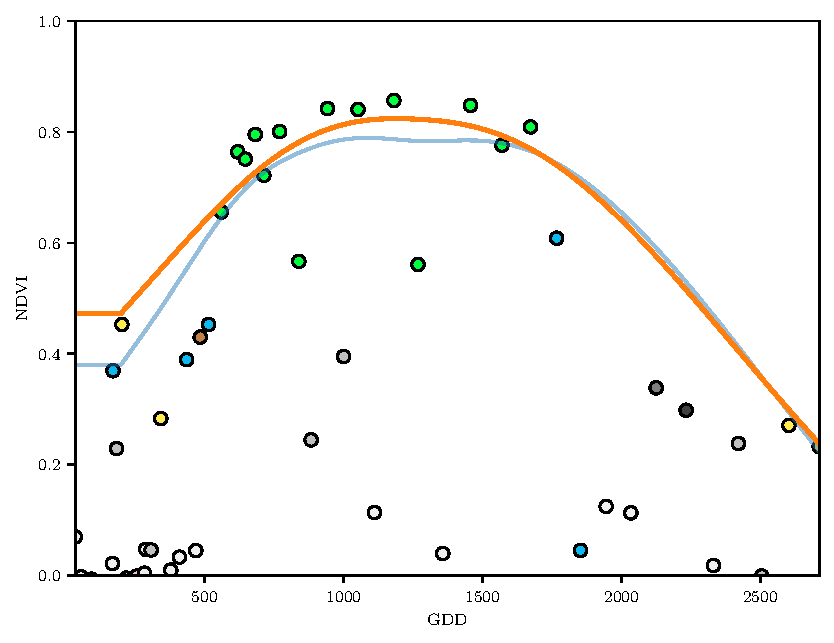
\includegraphics[width=\textwidth]{step_plot/2017-204_ndvi_scl.pdf}
		\vspace{-20pt}
		\caption[Now also consider other SCL-classes]%
		{\footnotesize Now also consider other SCL-classes}    
		\label{fig:step_plot/2017-204_ndvi_scl.pdf}
	\end{subfigure}

	\vskip\baselineskip
	\begin{subfigure}[b]{0.42\textwidth}   
		\centering 
		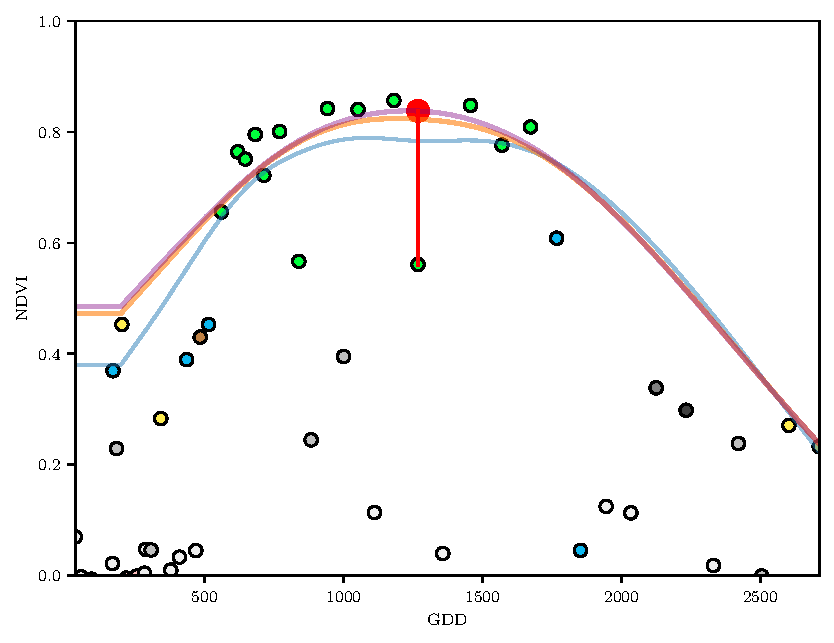
\includegraphics[width=\textwidth]{step_plot/2017-205_show_res.pdf}
		\vspace{-20pt}
		\caption[OOB estim. for each point using SCL45]%
		{{\footnotesize OOB estim. for each point using SCL45}}    
		\label{fig:step_plot/2017-205_show_res.pdf}
	\end{subfigure}
	\hfill
	\begin{subfigure}[b]{0.42\textwidth}   
		\centering 
		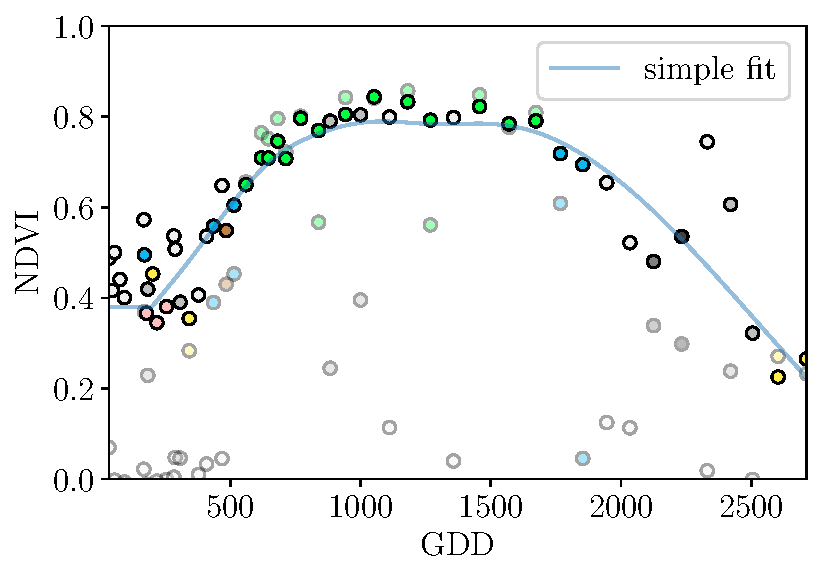
\includegraphics[width=\textwidth]{step_plot/2017-206_corr.pdf}
		\vspace{-20pt}
		\caption[Correct NDVI]%
		{\footnotesize Correct NDVI}    
		\label{fig:step_plot/2017-206_corr.pdf}
	\end{subfigure}

	\vskip\baselineskip
	\begin{subfigure}[b]{0.42\textwidth}   
		\centering 
		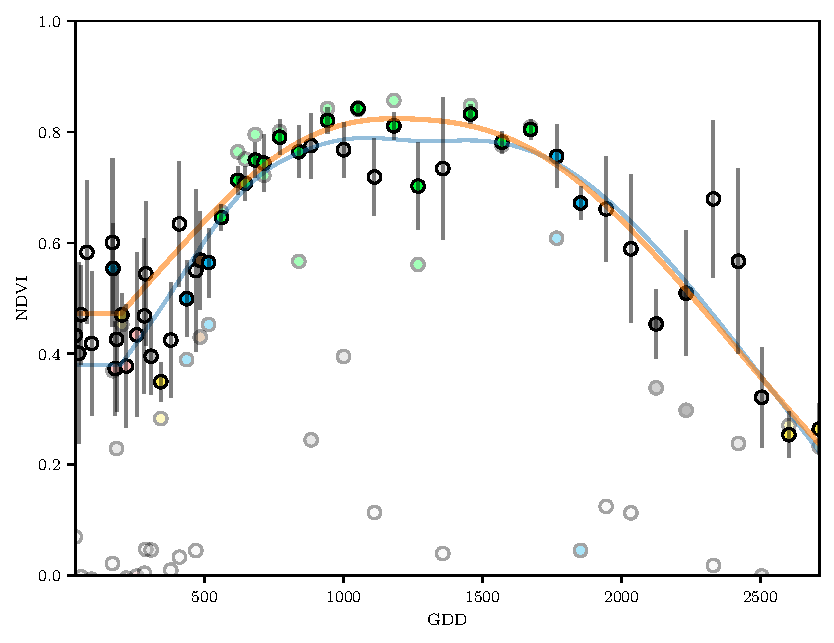
\includegraphics[width=\textwidth]{step_plot/2017-207_uncert.pdf}
		\vspace{-20pt}
		\caption[Estimate absolute errors]%
		{{\footnotesize Estimate absolute errors via statistical model}}    
		\label{fig:step_plot/2017-207_uncert.pdf}
	\end{subfigure}
	\hfill
	\begin{subfigure}[b]{0.42\textwidth}   
		\centering 
		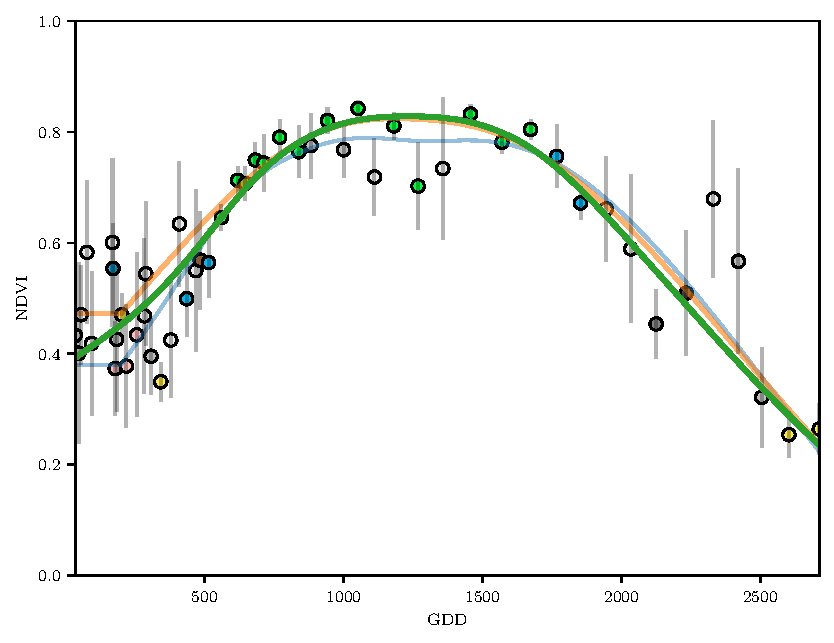
\includegraphics[width=\textwidth]{step_plot/2017-208_corr_itpl_rew.pdf}
		\vspace{-20pt}
		\caption[Interpolation (SS) on weights derived from uncertainties.]%
		{\footnotesize Robust interpolation on weights derived from uncertainties.}    
		\label{fig:step_plot/2017-208_corr_itpl_rew.pdf}
	\end{subfigure}
	\caption[Stepwise illustration of robust NDVI-Correction.]{Stepwise illustration of robust NDVI-Correction. For the color encoding of the SCL classes we refer to table~\ref{tab:satelite/scl_classes}.}
	\label{fig:step_plot_ndvi_corr}
\end{figure}



\begin{table}
	\begin{center}
		\caption{XXX RMSE of yield prediction}
		\small
		\begin{tabular}{lrrrrrrr}
\toprule
 & RF & OLS\textsuperscript{SCL} & OLS\textsuperscript{all} & MARS & GAM & LASSO & no corrections \\
\midrule
SS & {\cellcolor[HTML]{282828}} \color[HTML]{F1F1F1} 0.155 & {\cellcolor[HTML]{F1F1F1}} \color[HTML]{000000} 0.140 & {\cellcolor[HTML]{C9C9C9}} \color[HTML]{000000} 0.143 & {\cellcolor[HTML]{D6D6D6}} \color[HTML]{000000} 0.142 & {\cellcolor[HTML]{D6D6D6}} \color[HTML]{000000} 0.142 & {\cellcolor[HTML]{D6D6D6}} \color[HTML]{000000} 0.142 & {\cellcolor[HTML]{797979}} \color[HTML]{F1F1F1} 0.149 \\
SS\textsuperscript{rob} & {\cellcolor[HTML]{282828}} \color[HTML]{F1F1F1} 0.155 & {\cellcolor[HTML]{C9C9C9}} \color[HTML]{000000} 0.143 & {\cellcolor[HTML]{939393}} \color[HTML]{F1F1F1} 0.147 & {\cellcolor[HTML]{797979}} \color[HTML]{F1F1F1} 0.149 & {\cellcolor[HTML]{A0A0A0}} \color[HTML]{F1F1F1} 0.146 & {\cellcolor[HTML]{AEAEAE}} \color[HTML]{000000} 0.145 & {\cellcolor[HTML]{868686}} \color[HTML]{F1F1F1} 0.148 \\
DL & {\cellcolor[HTML]{1A1A1A}} \color[HTML]{F1F1F1} 0.156 & {\cellcolor[HTML]{5D5D5D}} \color[HTML]{F1F1F1} 0.151 & {\cellcolor[HTML]{505050}} \color[HTML]{F1F1F1} 0.152 & {\cellcolor[HTML]{505050}} \color[HTML]{F1F1F1} 0.152 & {\cellcolor[HTML]{797979}} \color[HTML]{F1F1F1} 0.149 & {\cellcolor[HTML]{797979}} \color[HTML]{F1F1F1} 0.149 & {\cellcolor[HTML]{000000}} \color[HTML]{F1F1F1} 0.158 \\
DL\textsuperscript{rob} & {\cellcolor[HTML]{0D0D0D}} \color[HTML]{F1F1F1} 0.157 & {\cellcolor[HTML]{434343}} \color[HTML]{F1F1F1} 0.153 & {\cellcolor[HTML]{505050}} \color[HTML]{F1F1F1} 0.152 & {\cellcolor[HTML]{AEAEAE}} \color[HTML]{000000} 0.145 & {\cellcolor[HTML]{868686}} \color[HTML]{F1F1F1} 0.148 & {\cellcolor[HTML]{6B6B6B}} \color[HTML]{F1F1F1} 0.150 & {\cellcolor[HTML]{0D0D0D}} \color[HTML]{F1F1F1} 0.157 \\
\bottomrule
\end{tabular}

		\label{tab:methods_vs_yieldprediction_relative}
		\normalsize
	\end{center}
\end{table}

\begin{table}
	\begin{center}
		\caption{XXX RMSE of yield prediction}
		\small
		\begin{tabular}{lrrrrrrr}
\toprule
 & RF & OLS-SCL & OLS-all & MARS & GAM & LASSO & no-correction \\
\midrule
ss & {\cellcolor[HTML]{F1F1F1}} \color[HTML]{000000} 0.431 & {\cellcolor[HTML]{000000}} \color[HTML]{F1F1F1} 0.486 & {\cellcolor[HTML]{272727}} \color[HTML]{F1F1F1} 0.477 & {\cellcolor[HTML]{141414}} \color[HTML]{F1F1F1} 0.481 & {\cellcolor[HTML]{1C1C1C}} \color[HTML]{F1F1F1} 0.479 & {\cellcolor[HTML]{141414}} \color[HTML]{F1F1F1} 0.481 & {\cellcolor[HTML]{878787}} \color[HTML]{F1F1F1} 0.455 \\
dl & {\cellcolor[HTML]{CFCFCF}} \color[HTML]{000000} 0.427 & {\cellcolor[HTML]{444444}} \color[HTML]{F1F1F1} 0.445 & {\cellcolor[HTML]{4A4A4A}} \color[HTML]{F1F1F1} 0.444 & {\cellcolor[HTML]{4A4A4A}} \color[HTML]{F1F1F1} 0.444 & {\cellcolor[HTML]{000000}} \color[HTML]{F1F1F1} 0.454 & {\cellcolor[HTML]{040404}} \color[HTML]{F1F1F1} 0.453 & {\cellcolor[HTML]{F1F1F1}} \color[HTML]{000000} 0.423 \\
ss-rob & {\cellcolor[HTML]{F1F1F1}} \color[HTML]{000000} 0.431 & {\cellcolor[HTML]{000000}} \color[HTML]{F1F1F1} 0.475 & {\cellcolor[HTML]{4E4E4E}} \color[HTML]{F1F1F1} 0.461 & {\cellcolor[HTML]{6A6A6A}} \color[HTML]{F1F1F1} 0.456 & {\cellcolor[HTML]{2D2D2D}} \color[HTML]{F1F1F1} 0.467 & {\cellcolor[HTML]{2B2B2B}} \color[HTML]{F1F1F1} 0.467 & {\cellcolor[HTML]{616161}} \color[HTML]{F1F1F1} 0.457 \\
dl-rob & {\cellcolor[HTML]{F1F1F1}} \color[HTML]{000000} 0.423 & {\cellcolor[HTML]{A2A2A2}} \color[HTML]{F1F1F1} 0.439 & {\cellcolor[HTML]{888888}} \color[HTML]{F1F1F1} 0.444 & {\cellcolor[HTML]{000000}} \color[HTML]{F1F1F1} 0.470 & {\cellcolor[HTML]{494949}} \color[HTML]{F1F1F1} 0.456 & {\cellcolor[HTML]{696969}} \color[HTML]{F1F1F1} 0.450 & {\cellcolor[HTML]{EBEBEB}} \color[HTML]{000000} 0.424 \\
\bottomrule
\end{tabular}

		\label{tab:methods_vs_yieldprediction_r2}
		\normalsize
	\end{center}
\end{table}

\lstinputlisting[title= R Summary of the NDVI correction model (c.f. equation \refeq{eq:corr_lm})]{tex/chapters/misc/lm_scl.txt}
\lstinputlisting[title= R Summary of the NDVI correction model (c.f. equation \refeq{eq:corr_lm_res})]{tex/chapters/misc/lm_scl_res.txt}


\todo[inline]{replace space before ref by tilda}
